\documentclass[1p]{elsarticle_modified}
%\bibliographystyle{elsarticle-num}

%\usepackage[colorlinks]{hyperref}
%\usepackage{abbrmath_seonhwa} %\Abb, \Ascr, \Acal ,\Abf, \Afrak
\usepackage{amsfonts}
\usepackage{amssymb}
\usepackage{amsmath}
\usepackage{amsthm}
\usepackage{scalefnt}
\usepackage{amsbsy}
\usepackage{kotex}
\usepackage{caption}
\usepackage{subfig}
\usepackage{color}
\usepackage{graphicx}
\usepackage{xcolor} %% white, black, red, green, blue, cyan, magenta, yellow
\usepackage{float}
\usepackage{setspace}
\usepackage{hyperref}

\usepackage{tikz}
\usetikzlibrary{arrows}

\usepackage{multirow}
\usepackage{array} % fixed length table
\usepackage{hhline}

%%%%%%%%%%%%%%%%%%%%%
\makeatletter
\renewcommand*\env@matrix[1][\arraystretch]{%
	\edef\arraystretch{#1}%
	\hskip -\arraycolsep
	\let\@ifnextchar\new@ifnextchar
	\array{*\c@MaxMatrixCols c}}
\makeatother %https://tex.stackexchange.com/questions/14071/how-can-i-increase-the-line-spacing-in-a-matrix
%%%%%%%%%%%%%%%

\usepackage[normalem]{ulem}

\newcommand{\msout}[1]{\ifmmode\text{\sout{\ensuremath{#1}}}\else\sout{#1}\fi}
%SOURCE: \msout is \stkout macro in https://tex.stackexchange.com/questions/20609/strikeout-in-math-mode

\newcommand{\cancel}[1]{
	\ifmmode
	{\color{red}\msout{#1}}
	\else
	{\color{red}\sout{#1}}
	\fi
}

\newcommand{\add}[1]{
	{\color{blue}\uwave{#1}}
}

\newcommand{\replace}[2]{
	\ifmmode
	{\color{red}\msout{#1}}{\color{blue}\uwave{#2}}
	\else
	{\color{red}\sout{#1}}{\color{blue}\uwave{#2}}
	\fi
}

\newcommand{\Sol}{\mathcal{S}} %segment
\newcommand{\D}{D} %diagram
\newcommand{\A}{\mathcal{A}} %arc


%%%%%%%%%%%%%%%%%%%%%%%%%%%%%5 test

\def\sl{\operatorname{\textup{SL}}(2,\Cbb)}
\def\psl{\operatorname{\textup{PSL}}(2,\Cbb)}
\def\quan{\mkern 1mu \triangleright \mkern 1mu}

\theoremstyle{definition}
\newtheorem{thm}{Theorem}[section]
\newtheorem{prop}[thm]{Proposition}
\newtheorem{lem}[thm]{Lemma}
\newtheorem{ques}[thm]{Question}
\newtheorem{cor}[thm]{Corollary}
\newtheorem{defn}[thm]{Definition}
\newtheorem{exam}[thm]{Example}
\newtheorem{rmk}[thm]{Remark}
\newtheorem{alg}[thm]{Algorithm}

\newcommand{\I}{\sqrt{-1}}
\begin{document}

%\begin{frontmatter}
%
%\title{Boundary parabolic representations of knots up to 8 crossings}
%
%%% Group authors per affiliation:
%\author{Yunhi Cho} 
%\address{Department of Mathematics, University of Seoul, Seoul, Korea}
%\ead{yhcho@uos.ac.kr}
%
%
%\author{Seonhwa Kim} %\fnref{s_kim}}
%\address{Center for Geometry and Physics, Institute for Basic Science, Pohang, 37673, Korea}
%\ead{ryeona17@ibs.re.kr}
%
%\author{Hyuk Kim}
%\address{Department of Mathematical Sciences, Seoul National University, Seoul 08826, Korea}
%\ead{hyukkim@snu.ac.kr}
%
%\author{Seokbeom Yoon}
%\address{Department of Mathematical Sciences, Seoul National University, Seoul, 08826,  Korea}
%\ead{sbyoon15@snu.ac.kr}
%
%\begin{abstract}
%We find all boundary parabolic representation of knots up to 8 crossings.
%
%\end{abstract}
%\begin{keyword}
%    \MSC[2010] 57M25 
%\end{keyword}
%
%\end{frontmatter}

%\linenumbers
%\tableofcontents
%
\newcommand\colored[1]{\textcolor{white}{\rule[-0.35ex]{0.8em}{1.4ex}}\kern-0.8em\color{red} #1}%
%\newcommand\colored[1]{\textcolor{white}{ #1}\kern-2.17ex	\textcolor{white}{ #1}\kern-1.81ex	\textcolor{white}{ #1}\kern-2.15ex\color{red}#1	}

{\Large $\underline{10_{59}~(K10a_{2})}$}

\setlength{\tabcolsep}{10pt}
\renewcommand{\arraystretch}{1.6}
\vspace{1cm}\begin{tabular}{m{100pt}>{\centering\arraybackslash}m{274pt}}
\multirow{5}{120pt}{
	\centering
	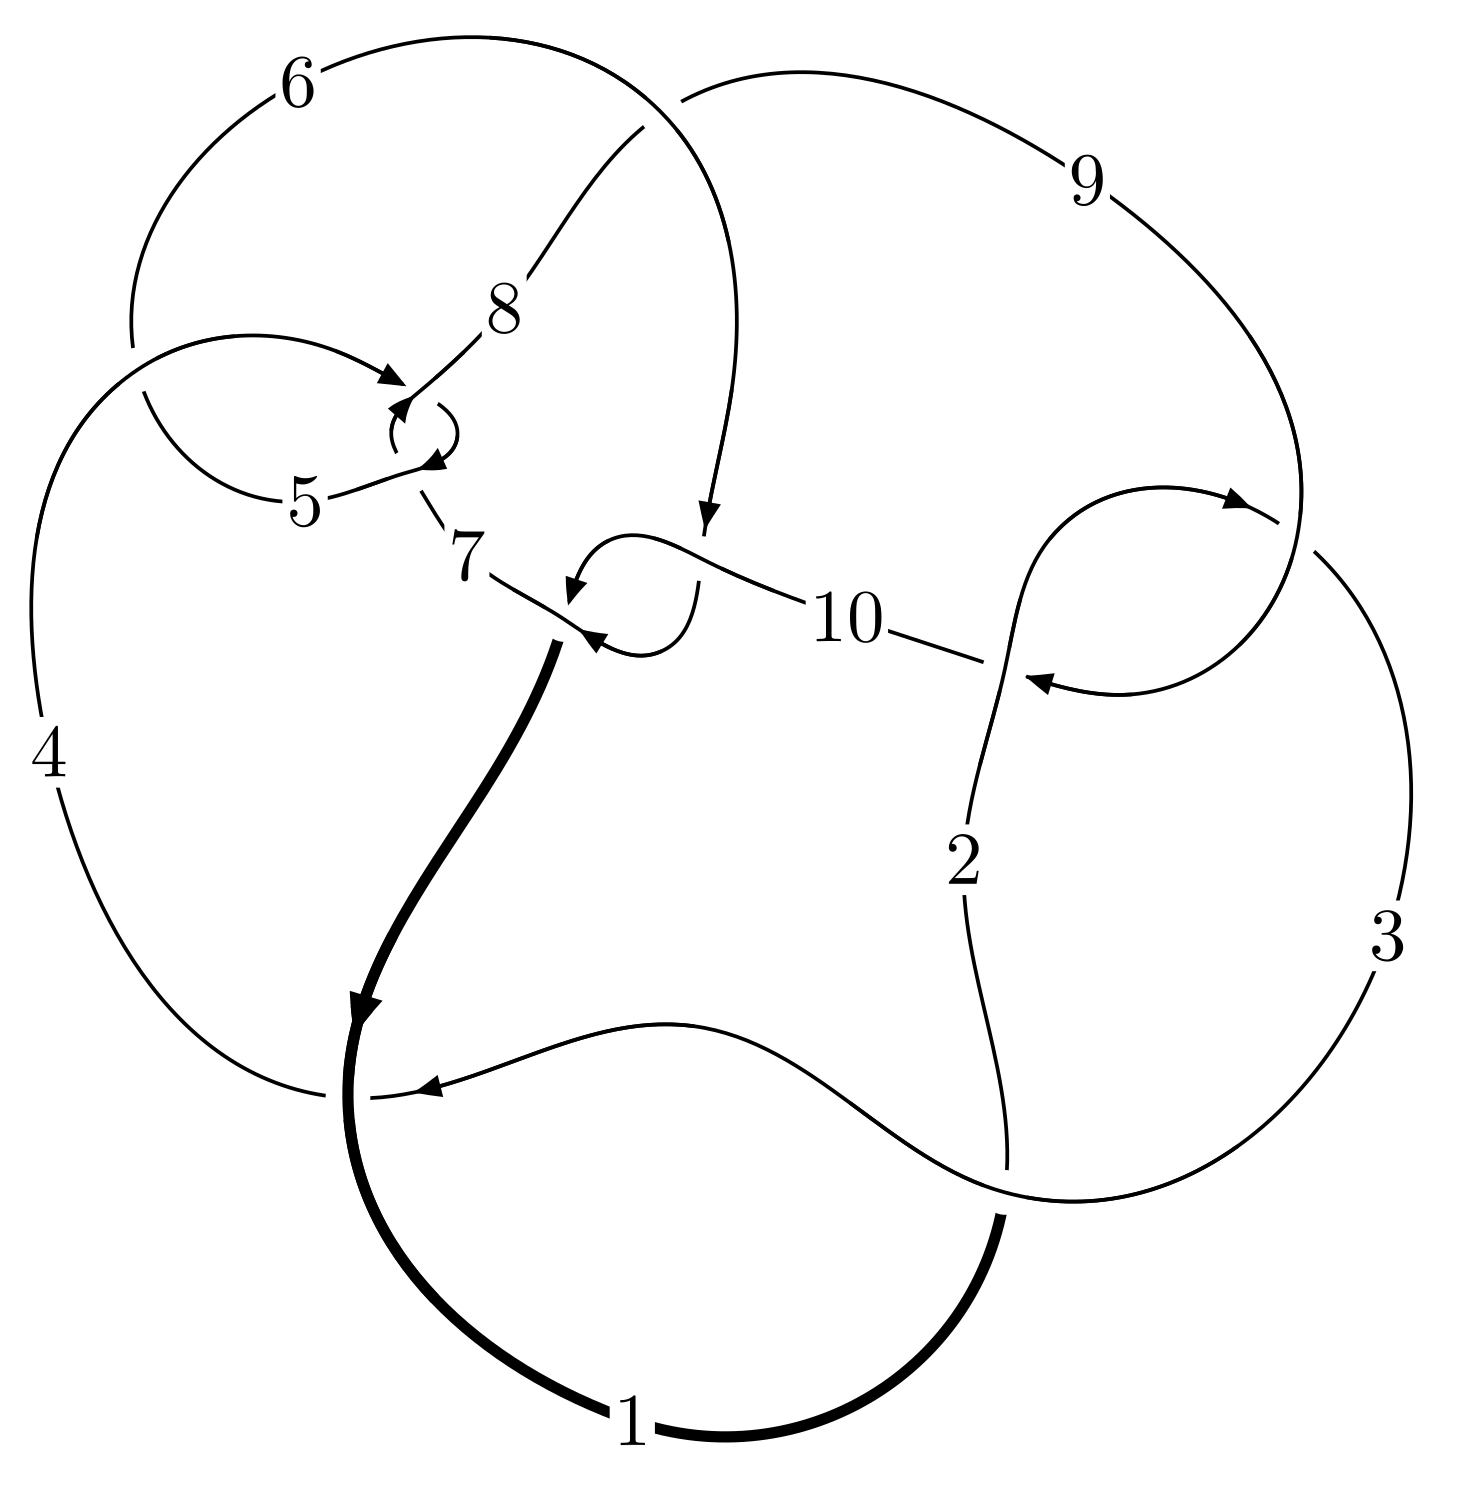
\includegraphics[width=112pt]{../../../GIT/diagram.site/Diagrams/png/143_10_59.png}\\
\ \ \ A knot diagram\footnotemark}&
\allowdisplaybreaks
\textbf{Linearized knot diagam} \\
\cline{2-2}
 &
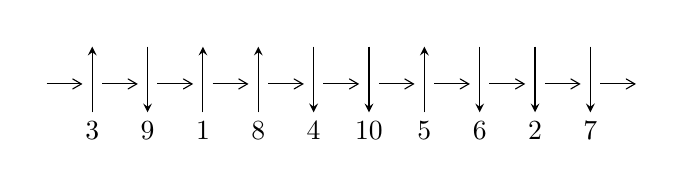
\begin{tikzpicture}[x=20pt, y=17pt]
	% nodes
	\node (C0) at (0, 0) {};
	\node (C1) at (1, 0) {};
	\node (C1U) at (1, +1) {};
	\node (C1D) at (1, -1) {3};

	\node (C2) at (2, 0) {};
	\node (C2U) at (2, +1) {};
	\node (C2D) at (2, -1) {9};

	\node (C3) at (3, 0) {};
	\node (C3U) at (3, +1) {};
	\node (C3D) at (3, -1) {1};

	\node (C4) at (4, 0) {};
	\node (C4U) at (4, +1) {};
	\node (C4D) at (4, -1) {8};

	\node (C5) at (5, 0) {};
	\node (C5U) at (5, +1) {};
	\node (C5D) at (5, -1) {4};

	\node (C6) at (6, 0) {};
	\node (C6U) at (6, +1) {};
	\node (C6D) at (6, -1) {10};

	\node (C7) at (7, 0) {};
	\node (C7U) at (7, +1) {};
	\node (C7D) at (7, -1) {5};

	\node (C8) at (8, 0) {};
	\node (C8U) at (8, +1) {};
	\node (C8D) at (8, -1) {6};

	\node (C9) at (9, 0) {};
	\node (C9U) at (9, +1) {};
	\node (C9D) at (9, -1) {2};

	\node (C10) at (10, 0) {};
	\node (C10U) at (10, +1) {};
	\node (C10D) at (10, -1) {7};
	\node (C11) at (11, 0) {};

	% arrows
	\draw[->,>={angle 60}]
	(C0) edge (C1) (C1) edge (C2) (C2) edge (C3) (C3) edge (C4) (C4) edge (C5) (C5) edge (C6) (C6) edge (C7) (C7) edge (C8) (C8) edge (C9) (C9) edge (C10) (C10) edge (C11) ;	\draw[->,>=stealth]
	(C1D) edge (C1U) (C2U) edge (C2D) (C3D) edge (C3U) (C4D) edge (C4U) (C5U) edge (C5D) (C6U) edge (C6D) (C7D) edge (C7U) (C8U) edge (C8D) (C9U) edge (C9D) (C10U) edge (C10D) ;
	\end{tikzpicture} \\
\hhline{~~} \\& 
\textbf{Solving Sequence} \\ \cline{2-2} 
 &
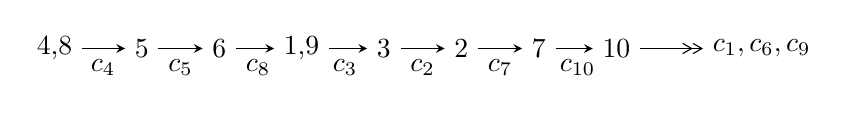
\begin{tikzpicture}[x=28pt, y=7pt]
	% node
	\node (A0) at (-1/8, 0) {4,8};
	\node (A1) at (1, 0) {5};
	\node (A2) at (2, 0) {6};
	\node (A3) at (49/16, 0) {1,9};
	\node (A4) at (33/8, 0) {3};
	\node (A5) at (41/8, 0) {2};
	\node (A6) at (49/8, 0) {7};
	\node (A7) at (57/8, 0) {10};
	\node (C1) at (1/2, -1) {$c_{4}$};
	\node (C2) at (3/2, -1) {$c_{5}$};
	\node (C3) at (5/2, -1) {$c_{8}$};
	\node (C4) at (29/8, -1) {$c_{3}$};
	\node (C5) at (37/8, -1) {$c_{2}$};
	\node (C6) at (45/8, -1) {$c_{7}$};
	\node (C7) at (53/8, -1) {$c_{10}$};
	\node (A8) at (9, 0) {$c_{1},c_{6},c_{9}$};

	% edge
	\draw[->,>=stealth]	
	(A0) edge (A1) (A1) edge (A2) (A2) edge (A3) (A3) edge (A4) (A4) edge (A5) (A5) edge (A6) (A6) edge (A7) ;
	\draw[->>,>={angle 60}]	
	(A7) edge (A8);
\end{tikzpicture} \\ 

\end{tabular} \\

\footnotetext{
The image of knot diagram is generated by the software ``\textbf{Draw programme}" developed by Andrew Bartholomew(\url{http://www.layer8.co.uk/maths/draw/index.htm\#Running-draw}), where we modified some parts for our purpose(\url{https://github.com/CATsTAILs/LinksPainter}).
}\phantom \\ \newline 
\centering \textbf{Ideals for irreducible components\footnotemark of $X_{\text{par}}$} 
 
\begin{align*}
I^u_{1}&=\langle 
u^{35}-4 u^{34}+\cdots+2 b-4,\;-6 u^{35}+17 u^{34}+\cdots+2 a+7,\;u^{36}-3 u^{35}+\cdots-2 u+1\rangle \\
I^u_{2}&=\langle 
b+u,\;a+1,\;u^2+u+1\rangle \\
I^u_{3}&=\langle 
u^2+b,\;- u^2+a-1,\;u^5+u^3+u-1\rangle \\
I^u_{4}&=\langle 
b- u-1,\;a+u,\;u^2+u+1\rangle \\
\\
\end{align*}
\raggedright * 4 irreducible components of $\dim_{\mathbb{C}}=0$, with total 45 representations.\\
\footnotetext{All coefficients of polynomials are rational numbers. But the coefficients are sometimes approximated in decimal forms when there is not enough margin.}
\newpage
\renewcommand{\arraystretch}{1}
\centering \section*{I. $I^u_{1}= \langle u^{35}-4 u^{34}+\cdots+2 b-4,\;-6 u^{35}+17 u^{34}+\cdots+2 a+7,\;u^{36}-3 u^{35}+\cdots-2 u+1 \rangle$}
\flushleft \textbf{(i) Arc colorings}\\
\begin{tabular}{m{7pt} m{180pt} m{7pt} m{180pt} }
\flushright $a_{4}=$&$\begin{pmatrix}1\\0\end{pmatrix}$ \\
\flushright $a_{8}=$&$\begin{pmatrix}0\\u\end{pmatrix}$ \\
\flushright $a_{5}=$&$\begin{pmatrix}1\\- u^2\end{pmatrix}$ \\
\flushright $a_{6}=$&$\begin{pmatrix}u^2+1\\- u^2\end{pmatrix}$ \\
\flushright $a_{1}=$&$\begin{pmatrix}3 u^{35}-\frac{17}{2} u^{34}+\cdots+\frac{13}{2} u-\frac{7}{2}\\-\frac{1}{2} u^{35}+2 u^{34}+\cdots-\frac{3}{2} u+2\end{pmatrix}$ \\
\flushright $a_{9}=$&$\begin{pmatrix}- u^5-2 u^3- u\\u^5+u^3+u\end{pmatrix}$ \\
\flushright $a_{3}=$&$\begin{pmatrix}-\frac{1}{2} u^{34}+u^{33}+\cdots-\frac{1}{2} u-\frac{1}{2}\\\frac{1}{2} u^{35}- u^{34}+\cdots-\frac{1}{2} u^2+\frac{3}{2} u\end{pmatrix}$ \\
\flushright $a_{2}=$&$\begin{pmatrix}\frac{1}{2} u^{35}-\frac{3}{2} u^{34}+\cdots-\frac{3}{2} u^2-\frac{1}{2}\\\frac{1}{2} u^{35}- u^{34}+\cdots-\frac{1}{2} u^2+\frac{3}{2} u\end{pmatrix}$ \\
\flushright $a_{7}=$&$\begin{pmatrix}- u\\u^3+u\end{pmatrix}$ \\
\flushright $a_{10}=$&$\begin{pmatrix}2 u^{35}-\frac{9}{2} u^{34}+\cdots+\frac{7}{2} u-\frac{5}{2}\\-\frac{3}{2} u^{35}+4 u^{34}+\cdots-\frac{3}{2} u+2\end{pmatrix}$\\&\end{tabular}
\flushleft \textbf{(ii) Obstruction class $= -1$}\\~\\
\flushleft \textbf{(iii) Cusp Shapes $= -\frac{13}{2} u^{35}+18 u^{34}+\cdots-\frac{11}{2} u-2$}\\~\\
\newpage\renewcommand{\arraystretch}{1}
\flushleft \textbf{(iv) u-Polynomials at the component}\newline \\
\begin{tabular}{m{50pt}|m{274pt}}
Crossings & \hspace{64pt}u-Polynomials at each crossing \\
\hline $$\begin{aligned}c_{1},c_{3}\end{aligned}$$&$\begin{aligned}
&u^{36}-11 u^{35}+\cdots-4 u+1
\end{aligned}$\\
\hline $$\begin{aligned}c_{2},c_{9}\end{aligned}$$&$\begin{aligned}
&u^{36}-3 u^{35}+\cdots-4 u+1
\end{aligned}$\\
\hline $$\begin{aligned}c_{4},c_{7}\end{aligned}$$&$\begin{aligned}
&u^{36}+3 u^{35}+\cdots+2 u+1
\end{aligned}$\\
\hline $$\begin{aligned}c_{5}\end{aligned}$$&$\begin{aligned}
&u^{36}+19 u^{35}+\cdots+4 u+1
\end{aligned}$\\
\hline $$\begin{aligned}c_{6},c_{10}\end{aligned}$$&$\begin{aligned}
&u^{36}-4 u^{35}+\cdots-48 u+16
\end{aligned}$\\
\hline $$\begin{aligned}c_{8}\end{aligned}$$&$\begin{aligned}
&u^{36}-3 u^{35}+\cdots-26 u+17
\end{aligned}$\\
\hline
\end{tabular}\\~\\
\newpage\renewcommand{\arraystretch}{1}
\flushleft \textbf{(v) Riley Polynomials at the component}\newline \\
\begin{tabular}{m{50pt}|m{274pt}}
Crossings & \hspace{64pt}Riley Polynomials at each crossing \\
\hline $$\begin{aligned}c_{1},c_{3}\end{aligned}$$&$\begin{aligned}
&y^{36}+31 y^{35}+\cdots+196 y+1
\end{aligned}$\\
\hline $$\begin{aligned}c_{2},c_{9}\end{aligned}$$&$\begin{aligned}
&y^{36}+11 y^{35}+\cdots+4 y+1
\end{aligned}$\\
\hline $$\begin{aligned}c_{4},c_{7}\end{aligned}$$&$\begin{aligned}
&y^{36}+19 y^{35}+\cdots+4 y+1
\end{aligned}$\\
\hline $$\begin{aligned}c_{5}\end{aligned}$$&$\begin{aligned}
&y^{36}- y^{35}+\cdots-12 y+1
\end{aligned}$\\
\hline $$\begin{aligned}c_{6},c_{10}\end{aligned}$$&$\begin{aligned}
&y^{36}-20 y^{35}+\cdots-128 y+256
\end{aligned}$\\
\hline $$\begin{aligned}c_{8}\end{aligned}$$&$\begin{aligned}
&y^{36}-21 y^{35}+\cdots+5682 y+289
\end{aligned}$\\
\hline
\end{tabular}\\~\\
\newpage\flushleft \textbf{(vi) Complex Volumes and Cusp Shapes}
$$\begin{array}{c|c|c}  
\text{Solutions to }I^u_{1}& \I (\text{vol} + \sqrt{-1}CS) & \text{Cusp shape}\\
 \hline 
\begin{aligned}
u &= -0.387195 + 0.859809 I \\
a &= \phantom{-}0.864957 + 0.109414 I \\
b &= -0.0189081 + 0.0958332 I\end{aligned}
 & -0.34130 - 1.65777 I & -2.55644 + 4.36495 I \\ \hline\begin{aligned}
u &= -0.387195 - 0.859809 I \\
a &= \phantom{-}0.864957 - 0.109414 I \\
b &= -0.0189081 - 0.0958332 I\end{aligned}
 & -0.34130 + 1.65777 I & -2.55644 - 4.36495 I \\ \hline\begin{aligned}
u &= -0.729583 + 0.777572 I \\
a &= -1.03050 + 1.01725 I \\
b &= \phantom{-}0.317863 - 1.274650 I\end{aligned}
 & -1.45237 - 5.42060 I & -4.83818 + 6.67480 I \\ \hline\begin{aligned}
u &= -0.729583 - 0.777572 I \\
a &= -1.03050 - 1.01725 I \\
b &= \phantom{-}0.317863 + 1.274650 I\end{aligned}
 & -1.45237 + 5.42060 I & -4.83818 - 6.67480 I \\ \hline\begin{aligned}
u &= \phantom{-}0.859716 + 0.267248 I \\
a &= -0.901846 + 1.060320 I \\
b &= \phantom{-}0.44242 - 1.51885 I\end{aligned}
 & -4.44713 - 8.11971 I & -3.47630 + 5.34748 I \\ \hline\begin{aligned}
u &= \phantom{-}0.859716 - 0.267248 I \\
a &= -0.901846 - 1.060320 I \\
b &= \phantom{-}0.44242 + 1.51885 I\end{aligned}
 & -4.44713 + 8.11971 I & -3.47630 - 5.34748 I \\ \hline\begin{aligned}
u &= \phantom{-}0.849597 + 0.216556 I \\
a &= \phantom{-}0.853721 - 0.852880 I \\
b &= -0.173950 + 1.239740 I\end{aligned}
 & -5.28539 - 2.14662 I & -5.02569 + 0.44253 I \\ \hline\begin{aligned}
u &= \phantom{-}0.849597 - 0.216556 I \\
a &= \phantom{-}0.853721 + 0.852880 I \\
b &= -0.173950 - 1.239740 I\end{aligned}
 & -5.28539 + 2.14662 I & -5.02569 - 0.44253 I \\ \hline\begin{aligned}
u &= -0.551728 + 0.987777 I \\
a &= -0.415426 - 1.128760 I \\
b &= \phantom{-}0.676359 - 0.193589 I\end{aligned}
 & \phantom{-}1.29309 - 3.12534 I & \phantom{-}1.43285 + 2.16786 I \\ \hline\begin{aligned}
u &= -0.551728 - 0.987777 I \\
a &= -0.415426 + 1.128760 I \\
b &= \phantom{-}0.676359 + 0.193589 I\end{aligned}
 & \phantom{-}1.29309 + 3.12534 I & \phantom{-}1.43285 - 2.16786 I\\
 \hline 
 \end{array}$$\newpage$$\begin{array}{c|c|c}  
\text{Solutions to }I^u_{1}& \I (\text{vol} + \sqrt{-1}CS) & \text{Cusp shape}\\
 \hline 
\begin{aligned}
u &= -0.587634 + 0.555787 I \\
a &= -0.996846 + 0.434125 I \\
b &= \phantom{-}0.801082 - 0.030150 I\end{aligned}
 & \phantom{-}2.54802 - 1.41982 I & \phantom{-}3.82315 + 3.52465 I \\ \hline\begin{aligned}
u &= -0.587634 - 0.555787 I \\
a &= -0.996846 - 0.434125 I \\
b &= \phantom{-}0.801082 + 0.030150 I\end{aligned}
 & \phantom{-}2.54802 + 1.41982 I & \phantom{-}3.82315 - 3.52465 I \\ \hline\begin{aligned}
u &= -0.424101 + 1.130320 I \\
a &= \phantom{-}1.47023 + 1.05531 I \\
b &= \phantom{-}0.079663 + 1.259790 I\end{aligned}
 & -4.09621 - 1.05243 I & -6.63369 + 0.71979 I \\ \hline\begin{aligned}
u &= -0.424101 - 1.130320 I \\
a &= \phantom{-}1.47023 - 1.05531 I \\
b &= \phantom{-}0.079663 - 1.259790 I\end{aligned}
 & -4.09621 + 1.05243 I & -6.63369 - 0.71979 I \\ \hline\begin{aligned}
u &= \phantom{-}0.515700 + 1.111390 I \\
a &= -1.30481 + 0.95936 I \\
b &= \phantom{-}1.199870 + 0.507968 I\end{aligned}
 & -0.65138 + 7.27213 I & -2.75984 - 7.42786 I \\ \hline\begin{aligned}
u &= \phantom{-}0.515700 - 1.111390 I \\
a &= -1.30481 - 0.95936 I \\
b &= \phantom{-}1.199870 - 0.507968 I\end{aligned}
 & -0.65138 - 7.27213 I & -2.75984 + 7.42786 I \\ \hline\begin{aligned}
u &= \phantom{-}0.445924 + 1.144390 I \\
a &= \phantom{-}0.761539 - 0.451840 I \\
b &= -0.595300 + 0.157343 I\end{aligned}
 & -4.74271 + 4.00295 I & -9.23293 - 4.01986 I \\ \hline\begin{aligned}
u &= \phantom{-}0.445924 - 1.144390 I \\
a &= \phantom{-}0.761539 + 0.451840 I \\
b &= -0.595300 - 0.157343 I\end{aligned}
 & -4.74271 - 4.00295 I & -9.23293 + 4.01986 I \\ \hline\begin{aligned}
u &= -0.471044 + 1.134590 I \\
a &= -1.37055 - 1.28746 I \\
b &= \phantom{-}0.30745 - 1.38445 I\end{aligned}
 & -3.75883 - 6.78157 I & -5.67848 + 6.13587 I \\ \hline\begin{aligned}
u &= -0.471044 - 1.134590 I \\
a &= -1.37055 + 1.28746 I \\
b &= \phantom{-}0.30745 + 1.38445 I\end{aligned}
 & -3.75883 + 6.78157 I & -5.67848 - 6.13587 I\\
 \hline 
 \end{array}$$\newpage$$\begin{array}{c|c|c}  
\text{Solutions to }I^u_{1}& \I (\text{vol} + \sqrt{-1}CS) & \text{Cusp shape}\\
 \hline 
\begin{aligned}
u &= -0.024315 + 0.768307 I \\
a &= \phantom{-}1.47731 - 0.09368 I \\
b &= \phantom{-}0.090892 - 0.615872 I\end{aligned}
 & -1.10226 - 1.38558 I & -6.76484 + 3.92520 I \\ \hline\begin{aligned}
u &= -0.024315 - 0.768307 I \\
a &= \phantom{-}1.47731 + 0.09368 I \\
b &= \phantom{-}0.090892 + 0.615872 I\end{aligned}
 & -1.10226 + 1.38558 I & -6.76484 - 3.92520 I \\ \hline\begin{aligned}
u &= \phantom{-}0.264173 + 1.234870 I \\
a &= \phantom{-}0.373926 - 0.622707 I \\
b &= \phantom{-}0.32517 - 1.56431 I\end{aligned}
 & -9.31556 - 4.56904 I & -8.72559 + 2.82656 I \\ \hline\begin{aligned}
u &= \phantom{-}0.264173 - 1.234870 I \\
a &= \phantom{-}0.373926 + 0.622707 I \\
b &= \phantom{-}0.32517 + 1.56431 I\end{aligned}
 & -9.31556 + 4.56904 I & -8.72559 - 2.82656 I \\ \hline\begin{aligned}
u &= \phantom{-}0.304638 + 1.233790 I \\
a &= -0.105861 + 0.569620 I \\
b &= -0.119820 + 1.383530 I\end{aligned}
 & -9.88952 + 1.61524 I & -9.56754 - 2.32735 I \\ \hline\begin{aligned}
u &= \phantom{-}0.304638 - 1.233790 I \\
a &= -0.105861 - 0.569620 I \\
b &= -0.119820 - 1.383530 I\end{aligned}
 & -9.88952 - 1.61524 I & -9.56754 + 2.32735 I \\ \hline\begin{aligned}
u &= \phantom{-}0.636789 + 0.302809 I \\
a &= -1.62143 + 0.78351 I \\
b &= \phantom{-}1.017930 - 0.416218 I\end{aligned}
 & \phantom{-}1.68165 - 2.75426 I & \phantom{-}1.42028 + 4.13268 I \\ \hline\begin{aligned}
u &= \phantom{-}0.636789 - 0.302809 I \\
a &= -1.62143 - 0.78351 I \\
b &= \phantom{-}1.017930 + 0.416218 I\end{aligned}
 & \phantom{-}1.68165 + 2.75426 I & \phantom{-}1.42028 - 4.13268 I \\ \hline\begin{aligned}
u &= \phantom{-}0.549648 + 1.188840 I \\
a &= \phantom{-}1.80307 - 0.33069 I \\
b &= -0.278564 - 1.254500 I\end{aligned}
 & -8.19229 + 7.27945 I & -7.73458 - 3.93070 I \\ \hline\begin{aligned}
u &= \phantom{-}0.549648 - 1.188840 I \\
a &= \phantom{-}1.80307 + 0.33069 I \\
b &= -0.278564 + 1.254500 I\end{aligned}
 & -8.19229 - 7.27945 I & -7.73458 + 3.93070 I\\
 \hline 
 \end{array}$$\newpage$$\begin{array}{c|c|c}  
\text{Solutions to }I^u_{1}& \I (\text{vol} + \sqrt{-1}CS) & \text{Cusp shape}\\
 \hline 
\begin{aligned}
u &= \phantom{-}0.572738 + 1.180430 I \\
a &= -1.98873 + 0.46037 I \\
b &= \phantom{-}0.48742 + 1.57860 I\end{aligned}
 & -7.1856 + 13.3899 I & -6.02318 - 8.65555 I \\ \hline\begin{aligned}
u &= \phantom{-}0.572738 - 1.180430 I \\
a &= -1.98873 - 0.46037 I \\
b &= \phantom{-}0.48742 - 1.57860 I\end{aligned}
 & -7.1856 - 13.3899 I & -6.02318 + 8.65555 I \\ \hline\begin{aligned}
u &= \phantom{-}0.274519 + 0.624372 I \\
a &= -2.10757 + 0.21578 I \\
b &= \phantom{-}0.635668 + 1.038860 I\end{aligned}
 & -0.04793 + 2.91691 I & -3.21123 - 0.65680 I \\ \hline\begin{aligned}
u &= \phantom{-}0.274519 - 0.624372 I \\
a &= -2.10757 - 0.21578 I \\
b &= \phantom{-}0.635668 - 1.038860 I\end{aligned}
 & -0.04793 - 2.91691 I & -3.21123 + 0.65680 I \\ \hline\begin{aligned}
u &= -0.597841 + 0.093585 I \\
a &= -0.261177 + 0.245146 I \\
b &= \phantom{-}0.304766 + 1.198650 I\end{aligned}
 & -0.94199 + 2.63032 I & -1.44776 - 2.88489 I \\ \hline\begin{aligned}
u &= -0.597841 - 0.093585 I \\
a &= -0.261177 - 0.245146 I \\
b &= \phantom{-}0.304766 - 1.198650 I\end{aligned}
 & -0.94199 - 2.63032 I & -1.44776 + 2.88489 I\\
 \hline 
 \end{array}$$\newpage\newpage\renewcommand{\arraystretch}{1}
\centering \section*{II. $I^u_{2}= \langle b+u,\;a+1,\;u^2+u+1 \rangle$}
\flushleft \textbf{(i) Arc colorings}\\
\begin{tabular}{m{7pt} m{180pt} m{7pt} m{180pt} }
\flushright $a_{4}=$&$\begin{pmatrix}1\\0\end{pmatrix}$ \\
\flushright $a_{8}=$&$\begin{pmatrix}0\\u\end{pmatrix}$ \\
\flushright $a_{5}=$&$\begin{pmatrix}1\\u+1\end{pmatrix}$ \\
\flushright $a_{6}=$&$\begin{pmatrix}- u\\u+1\end{pmatrix}$ \\
\flushright $a_{1}=$&$\begin{pmatrix}-1\\- u\end{pmatrix}$ \\
\flushright $a_{9}=$&$\begin{pmatrix}-1\\0\end{pmatrix}$ \\
\flushright $a_{3}=$&$\begin{pmatrix}u+1\\- u-1\end{pmatrix}$ \\
\flushright $a_{2}=$&$\begin{pmatrix}0\\- u-1\end{pmatrix}$ \\
\flushright $a_{7}=$&$\begin{pmatrix}- u\\u+1\end{pmatrix}$ \\
\flushright $a_{10}=$&$\begin{pmatrix}-1\\- u\end{pmatrix}$\\&\end{tabular}
\flushleft \textbf{(ii) Obstruction class $= 1$}\\~\\
\flushleft \textbf{(iii) Cusp Shapes $= 8 u+1$}\\~\\
\newpage\renewcommand{\arraystretch}{1}
\flushleft \textbf{(iv) u-Polynomials at the component}\newline \\
\begin{tabular}{m{50pt}|m{274pt}}
Crossings & \hspace{64pt}u-Polynomials at each crossing \\
\hline $$\begin{aligned}c_{1},c_{2},c_{4}\\c_{5},c_{8}\end{aligned}$$&$\begin{aligned}
&u^2+u+1
\end{aligned}$\\
\hline $$\begin{aligned}c_{3},c_{7},c_{9}\end{aligned}$$&$\begin{aligned}
&u^2- u+1
\end{aligned}$\\
\hline $$\begin{aligned}c_{6},c_{10}\end{aligned}$$&$\begin{aligned}
&u^2
\end{aligned}$\\
\hline
\end{tabular}\\~\\
\newpage\renewcommand{\arraystretch}{1}
\flushleft \textbf{(v) Riley Polynomials at the component}\newline \\
\begin{tabular}{m{50pt}|m{274pt}}
Crossings & \hspace{64pt}Riley Polynomials at each crossing \\
\hline $$\begin{aligned}c_{1},c_{2},c_{3}\\c_{4},c_{5},c_{7}\\c_{8},c_{9}\end{aligned}$$&$\begin{aligned}
&y^2+y+1
\end{aligned}$\\
\hline $$\begin{aligned}c_{6},c_{10}\end{aligned}$$&$\begin{aligned}
&y^2
\end{aligned}$\\
\hline
\end{tabular}\\~\\
\newpage\flushleft \textbf{(vi) Complex Volumes and Cusp Shapes}
$$\begin{array}{c|c|c}  
\text{Solutions to }I^u_{2}& \I (\text{vol} + \sqrt{-1}CS) & \text{Cusp shape}\\
 \hline 
\begin{aligned}
u &= -0.500000 + 0.866025 I \\
a &= -1.00000\phantom{ +0.000000I} \\
b &= \phantom{-}0.500000 - 0.866025 I\end{aligned}
 & \phantom{-0.000000 } -4.05977 I & -3.00000 + 6.92820 I \\ \hline\begin{aligned}
u &= -0.500000 - 0.866025 I \\
a &= -1.00000\phantom{ +0.000000I} \\
b &= \phantom{-}0.500000 + 0.866025 I\end{aligned}
 & \phantom{-0.000000 -}4.05977 I & -3.00000 - 6.92820 I\\
 \hline 
 \end{array}$$\newpage\newpage\renewcommand{\arraystretch}{1}
\centering \section*{III. $I^u_{3}= \langle u^2+b,\;- u^2+a-1,\;u^5+u^3+u-1 \rangle$}
\flushleft \textbf{(i) Arc colorings}\\
\begin{tabular}{m{7pt} m{180pt} m{7pt} m{180pt} }
\flushright $a_{4}=$&$\begin{pmatrix}1\\0\end{pmatrix}$ \\
\flushright $a_{8}=$&$\begin{pmatrix}0\\u\end{pmatrix}$ \\
\flushright $a_{5}=$&$\begin{pmatrix}1\\- u^2\end{pmatrix}$ \\
\flushright $a_{6}=$&$\begin{pmatrix}u^2+1\\- u^2\end{pmatrix}$ \\
\flushright $a_{1}=$&$\begin{pmatrix}u^2+1\\- u^2\end{pmatrix}$ \\
\flushright $a_{9}=$&$\begin{pmatrix}- u^3-1\\1\end{pmatrix}$ \\
\flushright $a_{3}=$&$\begin{pmatrix}- u^4- u^2+1\\u^4\end{pmatrix}$ \\
\flushright $a_{2}=$&$\begin{pmatrix}- u^2+u+1\\u^4- u\end{pmatrix}$ \\
\flushright $a_{7}=$&$\begin{pmatrix}- u\\u^3+u\end{pmatrix}$ \\
\flushright $a_{10}=$&$\begin{pmatrix}u^2+u+1\\- u^3- u^2- u\end{pmatrix}$\\&\end{tabular}
\flushleft \textbf{(ii) Obstruction class $= -1$}\\~\\
\flushleft \textbf{(iii) Cusp Shapes $= -6$}\\~\\
\newpage\renewcommand{\arraystretch}{1}
\flushleft \textbf{(iv) u-Polynomials at the component}\newline \\
\begin{tabular}{m{50pt}|m{274pt}}
Crossings & \hspace{64pt}u-Polynomials at each crossing \\
\hline $$\begin{aligned}c_{1},c_{3}\end{aligned}$$&$\begin{aligned}
&u^5-2 u^4+3 u^3-2 u^2+u+1
\end{aligned}$\\
\hline $$\begin{aligned}c_{2},c_{4},c_{7}\\c_{9}\end{aligned}$$&$\begin{aligned}
&u^5+u^3+u+1
\end{aligned}$\\
\hline $$\begin{aligned}c_{5}\end{aligned}$$&$\begin{aligned}
&u^5+2 u^4+3 u^3+2 u^2+u-1
\end{aligned}$\\
\hline $$\begin{aligned}c_{6},c_{10}\end{aligned}$$&$\begin{aligned}
&(u+1)^5
\end{aligned}$\\
\hline $$\begin{aligned}c_{8}\end{aligned}$$&$\begin{aligned}
&u^5+u^3-2 u^2- u+2
\end{aligned}$\\
\hline
\end{tabular}\\~\\
\newpage\renewcommand{\arraystretch}{1}
\flushleft \textbf{(v) Riley Polynomials at the component}\newline \\
\begin{tabular}{m{50pt}|m{274pt}}
Crossings & \hspace{64pt}Riley Polynomials at each crossing \\
\hline $$\begin{aligned}c_{1},c_{3},c_{5}\end{aligned}$$&$\begin{aligned}
&y^5+2 y^4+3 y^3+6 y^2+5 y-1
\end{aligned}$\\
\hline $$\begin{aligned}c_{2},c_{4},c_{7}\\c_{9}\end{aligned}$$&$\begin{aligned}
&y^5+2 y^4+3 y^3+2 y^2+y-1
\end{aligned}$\\
\hline $$\begin{aligned}c_{6},c_{10}\end{aligned}$$&$\begin{aligned}
&(y-1)^5
\end{aligned}$\\
\hline $$\begin{aligned}c_{8}\end{aligned}$$&$\begin{aligned}
&y^5+2 y^4- y^3-6 y^2+9 y-4
\end{aligned}$\\
\hline
\end{tabular}\\~\\
\newpage\flushleft \textbf{(vi) Complex Volumes and Cusp Shapes}
$$\begin{array}{c|c|c}  
\text{Solutions to }I^u_{3}& \I (\text{vol} + \sqrt{-1}CS) & \text{Cusp shape}\\
 \hline 
\begin{aligned}
u &= -0.707729 + 0.841955 I \\
a &= \phantom{-}0.79199 - 1.19175 I \\
b &= \phantom{-}0.208008 + 1.191750 I\end{aligned}
 & -1.64493\phantom{ +0.000000I} & -6.00000\phantom{ +0.000000I} \\ \hline\begin{aligned}
u &= -0.707729 - 0.841955 I \\
a &= \phantom{-}0.79199 + 1.19175 I \\
b &= \phantom{-}0.208008 - 1.191750 I\end{aligned}
 & -1.64493\phantom{ +0.000000I} & -6.00000\phantom{ +0.000000I} \\ \hline\begin{aligned}
u &= \phantom{-}0.389287 + 1.070680 I \\
a &= \phantom{-}0.005198 + 0.833601 I \\
b &= \phantom{-}0.994802 - 0.833601 I\end{aligned}
 & -1.64493\phantom{ +0.000000I} & -6.00000\phantom{ +0.000000I} \\ \hline\begin{aligned}
u &= \phantom{-}0.389287 - 1.070680 I \\
a &= \phantom{-}0.005198 - 0.833601 I \\
b &= \phantom{-}0.994802 + 0.833601 I\end{aligned}
 & -1.64493\phantom{ +0.000000I} & -6.00000\phantom{ +0.000000I} \\ \hline\begin{aligned}
u &= \phantom{-}0.636883\phantom{ +0.000000I} \\
a &= \phantom{-}1.40562\phantom{ +0.000000I} \\
b &= -0.405620\phantom{ +0.000000I}\end{aligned}
 & -1.64493\phantom{ +0.000000I} & -6.00000\phantom{ +0.000000I}\\
 \hline 
 \end{array}$$\newpage\newpage\renewcommand{\arraystretch}{1}
\centering \section*{IV. $I^u_{4}= \langle b- u-1,\;a+u,\;u^2+u+1 \rangle$}
\flushleft \textbf{(i) Arc colorings}\\
\begin{tabular}{m{7pt} m{180pt} m{7pt} m{180pt} }
\flushright $a_{4}=$&$\begin{pmatrix}1\\0\end{pmatrix}$ \\
\flushright $a_{8}=$&$\begin{pmatrix}0\\u\end{pmatrix}$ \\
\flushright $a_{5}=$&$\begin{pmatrix}1\\u+1\end{pmatrix}$ \\
\flushright $a_{6}=$&$\begin{pmatrix}- u\\u+1\end{pmatrix}$ \\
\flushright $a_{1}=$&$\begin{pmatrix}- u\\u+1\end{pmatrix}$ \\
\flushright $a_{9}=$&$\begin{pmatrix}-1\\0\end{pmatrix}$ \\
\flushright $a_{3}=$&$\begin{pmatrix}2\\u\end{pmatrix}$ \\
\flushright $a_{2}=$&$\begin{pmatrix}u+2\\u\end{pmatrix}$ \\
\flushright $a_{7}=$&$\begin{pmatrix}- u\\u+1\end{pmatrix}$ \\
\flushright $a_{10}=$&$\begin{pmatrix}- u\\u+1\end{pmatrix}$\\&\end{tabular}
\flushleft \textbf{(ii) Obstruction class $= 1$}\\~\\
\flushleft \textbf{(iii) Cusp Shapes $= 0$}\\~\\
\newpage\renewcommand{\arraystretch}{1}
\flushleft \textbf{(iv) u-Polynomials at the component}\newline \\
\begin{tabular}{m{50pt}|m{274pt}}
Crossings & \hspace{64pt}u-Polynomials at each crossing \\
\hline $$\begin{aligned}c_{1},c_{2},c_{4}\\c_{5},c_{8}\end{aligned}$$&$\begin{aligned}
&u^2+u+1
\end{aligned}$\\
\hline $$\begin{aligned}c_{3},c_{7},c_{9}\end{aligned}$$&$\begin{aligned}
&u^2- u+1
\end{aligned}$\\
\hline $$\begin{aligned}c_{6},c_{10}\end{aligned}$$&$\begin{aligned}
&u^2
\end{aligned}$\\
\hline
\end{tabular}\\~\\
\newpage\renewcommand{\arraystretch}{1}
\flushleft \textbf{(v) Riley Polynomials at the component}\newline \\
\begin{tabular}{m{50pt}|m{274pt}}
Crossings & \hspace{64pt}Riley Polynomials at each crossing \\
\hline $$\begin{aligned}c_{1},c_{2},c_{3}\\c_{4},c_{5},c_{7}\\c_{8},c_{9}\end{aligned}$$&$\begin{aligned}
&y^2+y+1
\end{aligned}$\\
\hline $$\begin{aligned}c_{6},c_{10}\end{aligned}$$&$\begin{aligned}
&y^2
\end{aligned}$\\
\hline
\end{tabular}\\~\\
\newpage\flushleft \textbf{(vi) Complex Volumes and Cusp Shapes}
$$\begin{array}{c|c|c}  
\text{Solutions to }I^u_{4}& \I (\text{vol} + \sqrt{-1}CS) & \text{Cusp shape}\\
 \hline 
\begin{aligned}
u &= -0.500000 + 0.866025 I \\
a &= \phantom{-}0.500000 - 0.866025 I \\
b &= \phantom{-}0.500000 + 0.866025 I\end{aligned}
 & \phantom{-0.000000 } 0 & \phantom{-0.000000 } 0 \\ \hline\begin{aligned}
u &= -0.500000 - 0.866025 I \\
a &= \phantom{-}0.500000 + 0.866025 I \\
b &= \phantom{-}0.500000 - 0.866025 I\end{aligned}
 & \phantom{-0.000000 } 0 & \phantom{-0.000000 } 0\\
 \hline 
 \end{array}$$\newpage
\newpage\renewcommand{\arraystretch}{1}
\centering \section*{ V. u-Polynomials}
\begin{tabular}{m{50pt}|m{274pt}}
Crossings & \hspace{64pt}u-Polynomials at each crossing \\
\hline $$\begin{aligned}c_{1}\end{aligned}$$&$\begin{aligned}
&((u^2+u+1)^2)(u^5-2 u^4+\cdots+u+1)(u^{36}-11 u^{35}+\cdots-4 u+1)
\end{aligned}$\\
\hline $$\begin{aligned}c_{2}\end{aligned}$$&$\begin{aligned}
&((u^2+u+1)^2)(u^5+u^3+u+1)(u^{36}-3 u^{35}+\cdots-4 u+1)
\end{aligned}$\\
\hline $$\begin{aligned}c_{3}\end{aligned}$$&$\begin{aligned}
&((u^2- u+1)^2)(u^5-2 u^4+\cdots+u+1)(u^{36}-11 u^{35}+\cdots-4 u+1)
\end{aligned}$\\
\hline $$\begin{aligned}c_{4}\end{aligned}$$&$\begin{aligned}
&((u^2+u+1)^2)(u^5+u^3+u+1)(u^{36}+3 u^{35}+\cdots+2 u+1)
\end{aligned}$\\
\hline $$\begin{aligned}c_{5}\end{aligned}$$&$\begin{aligned}
&((u^2+u+1)^2)(u^5+2 u^4+\cdots+u-1)(u^{36}+19 u^{35}+\cdots+4 u+1)
\end{aligned}$\\
\hline $$\begin{aligned}c_{6},c_{10}\end{aligned}$$&$\begin{aligned}
&u^4(u+1)^5(u^{36}-4 u^{35}+\cdots-48 u+16)
\end{aligned}$\\
\hline $$\begin{aligned}c_{7}\end{aligned}$$&$\begin{aligned}
&((u^2- u+1)^2)(u^5+u^3+u+1)(u^{36}+3 u^{35}+\cdots+2 u+1)
\end{aligned}$\\
\hline $$\begin{aligned}c_{8}\end{aligned}$$&$\begin{aligned}
&((u^2+u+1)^2)(u^5+u^3-2 u^2- u+2)(u^{36}-3 u^{35}+\cdots-26 u+17)
\end{aligned}$\\
\hline $$\begin{aligned}c_{9}\end{aligned}$$&$\begin{aligned}
&((u^2- u+1)^2)(u^5+u^3+u+1)(u^{36}-3 u^{35}+\cdots-4 u+1)
\end{aligned}$\\
\hline
\end{tabular}\newpage\renewcommand{\arraystretch}{1}
\centering \section*{ VI. Riley Polynomials}
\begin{tabular}{m{50pt}|m{274pt}}
Crossings & \hspace{64pt}Riley Polynomials at each crossing \\
\hline $$\begin{aligned}c_{1},c_{3}\end{aligned}$$&$\begin{aligned}
&(y^2+y+1)^2(y^5+2 y^4+3 y^3+6 y^2+5 y-1)\\
&\cdot(y^{36}+31 y^{35}+\cdots+196 y+1)
\end{aligned}$\\
\hline $$\begin{aligned}c_{2},c_{9}\end{aligned}$$&$\begin{aligned}
&((y^2+y+1)^2)(y^5+2 y^4+\cdots+y-1)(y^{36}+11 y^{35}+\cdots+4 y+1)
\end{aligned}$\\
\hline $$\begin{aligned}c_{4},c_{7}\end{aligned}$$&$\begin{aligned}
&((y^2+y+1)^2)(y^5+2 y^4+\cdots+y-1)(y^{36}+19 y^{35}+\cdots+4 y+1)
\end{aligned}$\\
\hline $$\begin{aligned}c_{5}\end{aligned}$$&$\begin{aligned}
&((y^2+y+1)^2)(y^5+2 y^4+\cdots+5 y-1)(y^{36}- y^{35}+\cdots-12 y+1)
\end{aligned}$\\
\hline $$\begin{aligned}c_{6},c_{10}\end{aligned}$$&$\begin{aligned}
&y^4(y-1)^5(y^{36}-20 y^{35}+\cdots-128 y+256)
\end{aligned}$\\
\hline $$\begin{aligned}c_{8}\end{aligned}$$&$\begin{aligned}
&(y^2+y+1)^2(y^5+2 y^4- y^3-6 y^2+9 y-4)\\
&\cdot(y^{36}-21 y^{35}+\cdots+5682 y+289)
\end{aligned}$\\
\hline
\end{tabular}
\vskip 2pc
\end{document}